%%%%%%%%%%%%%%%%%%%%%%%%%%%%%%%%%%%%%%%%%%%%%%%%%%%%%%%%%%%%%%%%
% Tipo de documento y paquetes
\documentclass[10pt]{book}
\usepackage{cdt/cdtProcesos}
\usepackage{cdt/calmecac}
\usepackage{subfigure}
\usepackage{appendix}
%\texttt{}
\lstset{
	basicstyle=\small\ttfamily, %footnotesize
	language=Java, %C, csh, Java, HTML, XML, sh, SQL, Delphi, C, C++
	keywordstyle=\color{blue},%
	tabsize=3,%
	frame=trBL,%
	commentstyle=\it\ttfamily,%
	numbers=left, numberstyle=\tiny,%
	stringstyle=\color{red}%
}

%%%%%%%%%%%%%%%%%%%%%%%%%%%%%%%%%%%%%%%%%%%%%%%%%%%%%%%%%%%%%%%%
% Datos del proyecto
    \sistema{Music Academy Course, Student and Service System}

    \documento{C1-PR}{Documentación de Procesos TO-BE y Requerimientos del Sistema}{\DRAFT{\today}} %\RELEASE{1.0}
    \fecha{\today}
    \proyecto[MACAD]{Music Academy Course and Student System}
    \organizacion{Organización Estudiantil para el Desarrollo de Proyectos}
    \author{Cédula de Análisis de la OEDP}
    \elaboro[OEDP]{Organización Estudiantil para el Desarrollo de Proyectos}
    \entrega{Francisco Isidoro Mera Torres}
     \aprobo[Product Owner]{Roger Schumann}


%%%%%%%%%%%%%%%%%%%%%%%%%%%%%%%%%%%%%%%%%%%%%%%%%%%%%%%%%%%%%%%%
% Presentación

    \title{\varProyecto}
    \subtitle {\varCveDocumento--\varDocumento}

    \setImgPortada[0.7]{calmecacTheme/footer}
    \setImgPleca[0.2]{calmecacTheme/footer}
    \setImgHeader{calmecacTheme/logoPar}{calmecacTheme/logoInp}
    \setImgLogo{calmecacTheme/headerInp}{calmecacTheme/headerPar}

%%%%%%%%%%%%%%%%%%%%%%%%%%%%%%%%%%%%%%%%%%%%%%%%%%%%%%%%%%%%%%%%
% Configuración

    %=========================================================
	% Para ocultar la información de control de cambios.
	\hideControlVersion

    %=========================================================
    % Para desactivar las referencias cruzadas.
  % \disablePersistence

%%%%%%%%%%%%%%%%%%%%%%%%%%%%%%%%%%%%%%%%%%%%%%%%%%%%%%%%%%%%%%%%
% Inicio del Documento
\begin{document}

    %=========================================================
    % Portada
    \thispagestyle{empty}
    \maketitle

    %=========================================================
    % Hoja de revisión
    \makeDocInfo
    \bigskip\\
    \makeObservaciones[3cm]
    \vspace{2cm}
    \makeFirmas

    %=========================================================
    % Indices del documento
    \frontmatter
    \tableofcontents
    \listoffigures
    \mainmatter
    
    
    \chapter{Introducción}
    % !TEX root = ../integrado.tex

\section{Propósito del Documento}

Este documento es el primer entregable del proyecto MACAD el cual está compuesto por la descripción de procesos TO-BE utilizando la notación B.P.M.N. en su segunda versión cuya especificación está con base en la notación U.M.L. por el O.M.G. Así mismo este documento contiene la especificación de los requerimientos iniciales del sistema asociados con un criterio que permitirá evaluar la satisfacción proporcionada por la implementación y puesta en producción del sistema \varSistema. El documento tiene como propósito establecer los acuerdos necesarios para la implementación del sistema. 


\section{Estructura}

El documento está compuesto por los siguientes capítulos:

\begin{itemize}
	\item El capítulo \ref{ch:analisis} contiene un análisis de la F.A.M.A. y su situación actual así como su visión y misión modificada con base en los servicios que puede llegar a brindar no sólo a estudiantes sino a artistas o empresas dedicadas al entretinimiento.
	
	\item En el capítulo \ref{ch:glosario} se encontrará un glosario de términos utilizados comúnmente en el negocio así como la incorporación de nuevos elementos que permitan alcanzar la visión y misión de la academia.
	
	\item En el capítulo \ref{ch:procesos} se encontrará la definición de los procesos que se modificarán para lograr alcanzar la visión de F.A.M.A. en un tiempo estimado de TANTOS AÑOS implementando un nuevo un modelo de negocio basado en suscripciones y de cola larga.
	
	\item En el capítulo \ref{ch:reqFunc} se encontrarán los requerimientos obtenidos a raíz de las juntas con el cliente y con base en el modelo de negocio que se utilizarán para implementar el sistema.
	
	\item En el capítulo \ref{ch:reqNoFunc} se encontrarán los requerimientos obtenidos a raíz de las limitaciones y restricciones en las que se deberá implementar el sistema MACAD.
	
	\item En el capítulo \ref{ch:criterio} se encontrarán los acuerdos para verificar que los requerimientos funcionales hayan sido cubiertos con el sistema, en su mayoría de forma satisfactoria.
\end{itemize}


\section{Nomenclatura}

Para apoyar a la lectura de este documento en esta sección se presentan la diferente nomenclatura utilizada en el documento para identificar : procesos, requerimientos y criterios de evaluación como se muestra en la siguiente tabla.


\begin{table}[hbtp!]
	\begin{center}
		\begin{tabular}{|p{0.7\textwidth}|}
			\hline
			\rowcolor{colorAgua}
			\begin{description}
				\item[PRXX] Indicador de un proceso principal del cual se derivan otros. Las XX indican un número entero que puede ir del \textit{00} hasta \textit{99} 
				\item[SPRXX] Indicador de un subproceso en donde se especifican las tareas que deben llevar a cabo 
				
				\item[RF-MM-XX] Indicador de los requerimientos funcionales. Las MM indican el módulo al que se asignó el requerimiento de acuerdo a a la necesidad que se va a cubrir. Las XX indican un número entero que puede ir del \textit{00} hasta \textit{99}.
				
				\item[RNF-XX] Indicador de los requerimientos no funcionales del sistema. Debido a que estos requerimientos tienden a restringir el desarrollo del sistema no tienen un módulo asociado.
				
				\item[CR-MM-XX] Indicador de criterios de evaluación para los requerimientos funcionales. Al igual que los requerimientos funcionales estos contienen la nomenclatura MM para indicar el módulo al que pertenece el criterio.
			\end{description}\\
			\hline
		\end{tabular}
	\end{center}
\end{table}




    
    \chapter{Análisis de la Empresa}
    \label{ch:analisis}
    % !TEX root = ../integrado.tex

\section{Contexto}

F.A.M.A. es una academia en donde se imparten cursos de actualización y capacitación en software especializado para el entretenimiento a escuelas (como el I.P.N.), personas en un rango de edad de 15 a 30 años y a empresas en esta área como lo es T.V. Azteca. Cuenta con profesionales egresados del I.P.N. y de escuelas privadas y sus instalaciones se encuentran dentro de la Ciudad de México en la colonia Santa María la Rivera delegación Cauhtémoc. Sus principales competidores son G. Martell y Fermatta, quienes llevan dominando este campo por algunos años. F.A.M.A. goza de un ambiente muy agradable para la enseñanza, el equipo mínimo necesario para impartir sus cursos y cuenta con un pequeña cabina en donde se pueden realizar prácticas profesionales o grabaciones profesionales a artistas o músicos. Actualmente sus convenios más fuertes son con la empresa alemana \href{https://www.steinberg.net/en/products/cubase/start.html}{Steinberg} y con una de las empresas fabricantes de los sintetizadores más populares en el mundo \href{https://www.arturia.com/}{Arturia}, estos convenios permiten la entrega de paquetes promocionales o de estudiante así como de la certificación que avala el uso del software de estas dos empresas, entre otras. Como se mencionó previamente los alumnos pueden ser desde personas que tengan curiosidad por las tecnologías involucradas en la producción musical, hasta empresas pertenecientes a la industria del entretenimiento.\\

F.A.M.A. está bajo la dirección de Roger Schumann, productor reconocido en la industria, quien ha externado en diferentes momentos su preocupación por mantener a la academia a flote a pesar de las dificultades a las que se enfrenta mes con mes(las cuales serán mencionadas en una sección posterior). La academia tampoco cuenta con una misión y visión que le permitan implementar estrategias para tener una mayor recepción de alumnos que deseen estudiar o aprender acerca de la música o las tecnologías involucradas en su producción. F.A.M.A. ha planteado y planeado programas de estudio, cursos y diplomados que permitan cubrir la necesidad de profesionistas o técnicos especializados en la rama de la producción musical y sus derivados, los cuales carecen de una validez oficial por las autoridades mexicanas, pero que gozan del reconocimiento por las empresas con las que se tiene convenio y ex alumnos que han tenido éxito al concluir sus estudios en esta academia. F.A.M.A. plantea la calidad sobre la cantidad y esto se ve reflejado en el precio que se debe pagar por los servicios que provee en comparación con sus principales competidores.

En las subsecuentes secciones se especificarán los procesos como actualmente se llevan a cabo así como el análisis de sus principales problemáticas y consecuencias.


\section{Organigrama}

La organización de F.A.M.A. se puede observar en la figura \ref{fig:organigrama}, en donde se destacará la existencia de tres roles principales que serán afectados por el sistema que se va a implementar. Cada rol tendrá una especificación que contendrá sus características, funciones y perfil. Se agregarán más roles actualmente, a excepción del alumno, no son trascendentales para la actividad de F.A.M.A. pero que se espera en un futuro utilicen el sistema o se vean afectados por su implementación. Estos roles son:
	\begin{itemize}
		\item Alumno.
		\item Músico.
		\item Banda Musical.
		\item Empresa de Entretenimiento.
	\end{itemize}


\begin{figure}[hbtp!]
	\begin{center}
		\fbox{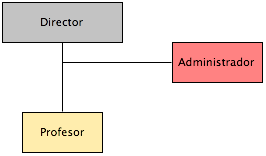
\includegraphics[width=0.5\textwidth]{analisis/images/organigrama}}
		\caption{Organigrama de F.A.M.A.}
		\label{fig:organigrama}
	\end{center}
\end{figure}

% !TEX root = ../integrado.tex

\begin{actor}{Director}{Director}{Persona al frente de la academia. Toma desiciones y evalúa las situaciones que mejoren el desempeño educativo de la academia así como la búsqueda de posibles usuarios para los servicios que ofrece F.A.M.A.}
\item[Funciones:]\cdtEmpty
	\begin{Citemize}
		\item Planificar los horarios y seleccionar los cursos a ofertar para un trimestre.
		\item Vigilar el desempeño de profesores y de alumnos.
		\item Planificar e implementar estrategias de crecimiento para F.A.M.A.	
	\end{Citemize}
	
\item[Perfil:]\cdtEmpty
	\begin{Citemize}
		\item Licenciatura.
		\item Responsable.
		\item Equitativo.
		\item Toma de Desiciones. 
	\end{Citemize}

\end{actor}

\begin{actor}{Administrador}{Administrador}{Persona encargada de los recursos financieros y recursos materiales de F.A.M.A. }
\item[Funciones:]\cdtEmpty
	\begin{Citemize}
		\item Gestionar los recursos financieros, materiales y espacios de F.A.M.A. y asignarlos a las áreas o espacios dentro de las instalaciones que 
		más lo requieran.
		\item Mantener el registro del pago de los alumnos así como implementar un mecanismo para que los alumnos que tienen constantes incidencias puedan permanecer en la academia. 
		\item Mantener el registro del pago de los profesores.
		\item Gestionar el 
	\end{Citemize}
\item[Perfil:]\cdtEmpty
	\begin{Citemize}
		\item Licenciatura.
		\item Responsable.
		\item Confiable.
	\end{Citemize}
\end{actor}


\begin{actor}{Profesor}{Profesor}{Persona encargada de transmitir conocimientos y resolver dudas a un grupo de personas reunidas en un lugar físico o virtual sobre uno o varios temas.}
\item[Funciones:]\cdtEmpty
	\begin{Citemize}
		\item Dar clase en un horario establecido.
		\item Resolver dudas.
		\item Evaluar a los alumnos.
		\item Preparar o mejorar el contenido de los cursos.	
	\end{Citemize}
\item[Perfil:]\cdtEmpty
	\begin{Citemize}
		\item Licenciatura o Técnico.
		\item Responsable.
		\item Proactivo.
	\end{Citemize}
\end{actor}

\begin{actor}{Alumno}{Alumno}{Persona interesada en adquirir servicios educativos de F.A.M.A.}
\item[Responsabilidades:]\cdtEmpty
	\begin{itemize}
		\item Asistir a clases.
		\item Presentar los exámenes correspondientes para concluir un curso, carrera o stack de tecnologías.
		\item Pagar a tiempo por el número de cursos que toma, carrera o stack de tecnologías.
	\end{itemize}
\item[Perfil:]No aplica.
\end{actor}

\begin{actor}{Musico}{Músico}{Persona que se dedica profesionalmente o de pasatiempo a la música y que desea utilizar alguno de los servicios ofertados por F.A.M.A.}
\item[Responsabilidades:]\cdtEmpty
	\begin{itemize}
		\item Mantenerse en contacto continúo con el \refElem{Administrador} para planificar citas, reuniones o grabaciones individuales.
		\item Calificar el servicio proporcionado.
	\end{itemize}
\item[Perfil:] No aplica.
\end{actor}


\begin{actor}{BandaMusical}{Banda Musical}{Grupo de personas que se dedican a la música de profesión o pasatiempo que desean utilizar alguno de los servicios ofertados por F.A.M.A.}
\item[Responsabilidades:]\cdtEmpty
	\begin{Citemize}
		\item Mantenerse en contacto continúo con el \refElem{Administrador} para planificar citas, reuniones o grabaciones.
		\item Calificar el servicio proporcionado.
	\end{Citemize}
\item[Perfil:]No aplica.
\end{actor}

\begin{actor}{Empresa}{Empresa}{Ente comercial que desea que su personal sea capacitado en el uso de una o varias tecnologías en específico relacionadas al entretenimiento.}
\item[Responsabilidades:]\cdtEmpty
	\begin{Citemize}
		\item Pagar por la inscripción y mensualidad de las personas que tomarán el curso o stack de tecnologías proporcionadas por F.A.M.A.
		\item Calificar el servicio proporcionado.
	\end{Citemize}
\item[Perfil:] No aplica.
\end{actor}

\begin{actor}{Proveedor}{Proveedor}{Ente comercial que se dedica a otorgarle a la academia algunos productos gratuitamente o por un pago menor al común por un convenio establecido con el \refElem{Director}}
\item[Responsabilidades:]\cdtEmpty
	\begin{Citemize}
		\item Mantenerse en contacto con el \refElem{Director} para proporcionarle productos.
		\item Dar las 
	\end{Citemize}
\end{actor}


    
  	\chapter{Glosario de Términos}
	\label{ch:glosario}
	% !TEX root = ../integrado.tex

En este capítulo se encuentran los diferentes términos de negocio comúnmente utilizados en la academia F.A.M.A. por el \refElem{Director}, \refElem{Administrador} y \refElem{Profesor} para comunicar ideas o plantear cambios o sugerencias a los cursos o servicios.

\section{Glosario de términos}

\begin{bGlosario}
	
	\bTerm[Alumnos]{tAlumno}{Alumno}{Persona que paga por tomar uno o varios cursos, o una carrera que F.A.M.A. ofrece.}
	
	\bTerm{tApuntes}{Apuntes}{Se conoce como apuntes a los contenidos de los diferentes temas que conforman a un curso.}
	
	\bTerm{tAsistencia}{Asistencia}{Es la acción que un Alumno realiza cuando toma su clase en la hora y fecha indicada para tal propósito.}
	
	\bTerm{tBandaMusical}{Banda Musical}{Grupo de personas que desean que se les grabe, edite o que produzca material discográfico digital o físico.}
	
	\bTerm{tCarrera}{Carrera}{Conjunto de cursos que tienen como propósito formar a profesionales aptos en una rama específica del conocimiento.}
	
	\bTerm{tCertificado}{Certificado}{Documento expedido cuando un alumno a concluido un curso con una calificación arriba del 80\%.}
	
	\bTerm{tCurso}{Curso}{Temas recopilados y planificados de forma secuencial para adquirir conocimiento sobre una materia en específico}
	
	\bTerm{tEmpresa}{Empresa}{Organización que paga por la capacitación de su personal en una o varias tecnologías en específico.}
	
	\bTerm{tEvaluacion}{Evaluación}{Al medio digital o escrito que pone a prueba los conocimientos adquiridos por un alumno durante un curso.}
	
	\bTerm{tHorarioDeDisponibilidad}{Horario de Disponibilidad}{Días y horas de la semana con las que un alumno cuenta para tomar clase en la academia de forma virtual o de forma presencial.}
	
	\bTerm{tLicencia}{Licencia}{Clave, llave o dispositivo que permite utilizar un determinado software o varios programas de un mismo desarrollador, por un periodo de tiempo limitado o ilimitado, esto con base en el convenio establecido con F.A.M.A.}
	
	\bTerm{tPago}{Pago}{Dinero que se da a la academia por un servicio, curso o carrera. }
	
	\bTerm{tProfesor}{Profesor}{Persona que domina un conjunto de conocimientos los cuales transmite a un grupo de personas.}

	\bTerm{tServicioDeCapacitacion}{Servicio de Capacitación}{Conjunto de acciones que se le brinda a una empresa para que su personal se actualice en el uso y manipulación de un conjunto de tecnologías en específico.}
	
	\bTerm{tServiciodeGrabacion}{Servicio de Grabación}{Conjunto de acciones que se le brinda a un músico o banda musical que les permitan tener material discográfico digital o físico grabado, editado o producido en las instalaciones de la academia.}
	 		
	\bTerm{tStack}{Stack de Tecnologías}{Conjunto de cursos que tienen como propósito enseñar a un alumno el uso y manejo de una tecnología en específico.}

\end{bGlosario}

	
	\chapter{Procesos AS-IS}
	\label{ch:procesosasis}	
	% !TEX root = ../integrado.tex



\section{Introducción}
En este capítulo se presenta el análisis correspondiente de los procesos AS-IS de F.A.M.A. Un proceso AS-IS es la descripción de las acciones o tareas llevadas a cabo actualmente por los diferentes participantes involucrados en el proceso de negocio. Esta descripción tiene como propósito apoyar al descubrimiento de problemáticas que impiden el crecimiento de la empresa así como la identificación de áreas de oportunidad que pudieran llegar a ser implementadas en el negocio parea mejorar los servicios o productos que se ofertan.


\section{Notación}

Los procesos de negocio en este capítulo son los más relevantes de F.A.M.A. y los cuales se toman como referencia para el análisis, diseño e implementación de un sistema que apoye en la resolución de las problemáticas a las que la academia se enfrenta. Cada proceso tiene su sección correspondiente presentando un resumen general del proceso así como su diagrama correspondiente. Los diagramas están basados en la notación especificada por la O.M.G. del Business Process Modeling Notation en su versión 2.0. Posterior a su resumen se expone una tabla de elementos que permiten la ejecución del proceso. Finalmente se enlista cada tarea o subproceso realizado por los participantes hasta la conclusión del proceso.

% !TEX root = ../integrado.tex


\begin{Proceso}{PR01}{Ejecución de Trimestre}{La academia F.A.M.A. organiza sus actividades en periodos de tres meses. En un inicio el \refElem{Director} notifica a los alumnos de la escuela un fecha propuesta para el inicio de actividades. Una vez llegada la fecha los alumnos se presentan a la academia en donde el Director solicita los horarios de disponibilidad de cada uno y selecciona los cursos que se impartirán en el trimestre. En todo momento durante la ejecución del trimestre el \refElem{Administrador} busca a los alumnos para solicitar el pago correspondiente a su inscripción, ya sea por los cursos que los alumnos toman o por su carrera inscrita. Mientras se ejecuta el trimestre, el \refElem{Director} busca patrocinios de diferentes empresas y también solicita licencias a su proveedor \textit{Yamaha México} }{\Pfig[1]{asis/images/PR01-TrimestreASIS}{PR01}{Ejecución del Trimestre}}
	
	\PRitem{Participantes}{\begin{Titemize}
		\Titem \refElem{Director}
		\Titem \refElem{Administrador}
		\Titem \refElem{Profesor}
		\Titem \refElem{Alumno}
		\Titem \refElem{Proveedor}
	\end{Titemize}}	
	\PRitem{Entradas}{\begin{Titemize}
			\Titem Cursos(\refElem{tCurso}).
			\Titem \refElem{tHorarioDeDisponibilidad}.
			\Titem \refElem{tLicencia}.
			\Titem \refElem{tPago}.
			\Titem \refElem{tAsistencia}.
		\end{Titemize}}
	\PRitem{Salidas}{\begin{Titemize}
		\Titem \refElem{tCertificado}.
		\Titem \refElem{tApuntes}.
		\Titem \refElem{tEvaluacion}. 
	\end{Titemize}}

\end{Proceso}


\begin{PDescripcion}
	\Ppaso[\EinicioTiempo] El proceso inicia cada tres meses. El \refElem{Director} notifica a los alumnos del inicio de un nuevo trimestre.
	\Ppaso[\PSubProceso]\cdtLabelTask{SPR01}{Especificar fechas de nuevo trimestre} El \refElem{Director} planifica el inicio y fin de un nuevo trimestre. Continúa con la tarea \cdtRefTask{SPR02}{Dar inicio a trimestre}.
	
	\Ppaso[\PSubProceso]\cdtLabelTask{SPR02}{Dar inicio a trimestre} El \refElem{Director} cita a los alumnos a asistir el día de inicio de trimestre.
	
	\Ppaso[\iCompuerta] Una vez iniciado el trimestre se realizarán paralelamente las actividades \cdtRefTask{SPR03}{Cobrar a alumnos}, \cdtRefTask{SPR04}{Definir cursos y horarios}, \cdtRefTask{SPR07}{Buscar patrocinios} y \cdtRefTask{SPR08}{Solicitar Licencia}
	
	\Ppaso[\PSubProceso] \cdtLabelTask{SPR03}{Cobrar a alumnos} El \refElem{Administrador} a lo largo del trimestre solicitará el cobro por los cursos inscritos por el alumno en el trimestre.
	
	\Ppaso[\PSubProceso] \cdtLabelTask{SPR04}{Definir cursos y horarios} El \refElem{Director} durante una clase solicitará a los alumnos su \refElem{tHorarioDeDisponibilidad} para poder planificar el horario semanal de los cursos. Así mismo seleccionará los cursos que se ofertarán aleatoriamente o siguiendo la secuencia de los cursos ofertados el trimestre pasado. Continua con el sub proceso \cdtRefTask{SPR05}{Iniciar clases}.
	
	\Ppaso[\PSubProceso] \cdtLabelTask{SPR07}{Buscar patrocinios} El \refElem{Director} a lo largo del trimestre y de forma paralela buscará obtener patrocinios de diferentes empresas que puedan otorgar licencias estudiantiles o precios especiales de productos que puedan ser otorgadas a los alumnos. Esta tarea no tiene continuación.
	
	\Ppaso[\PSubProceso] \cdtLabelTask{SPR08}{Solicitar Licencia} El \refElem{Director} a lo largo del trimestre solicitará a su \refElem{Proveedor} un conjunto de licencias de software para los estudiantes. Está tarea no tiene continuación.
	
	\Ppaso[\PSubProceso] \cdtLabelTask{SPR05}{Iniciar Clases} El \refElem{Director} marca el inicio de las clases.
	
	\Ppaso[\iCompuerta] Una vez iniciadas las clases se llevarán a cabo las siguientes tareas en paralelo: \cdtRefTask{SPR06}{Dar Clase}, \cdtRefTask{SPR09}{Vigilar desempeño de profesores}.
	
	\Ppaso[\PSubProceso] \cdtLabelTask{SPR06}{Dar Clase} El \refElem{Profesor} le proporcionará apuntes a los alumnos inscritos en su curso por medio de la plataforma de Moodle o por medios escritos. Este evento sucederá hasta que los temas hayan sido cubiertos en su totalidad o al 80\%. Concluida este subproceso se continua con \cdtRefTask{SPR07}{Evaluar Alumnos}.
	
	\Ppaso[\PSubProceso] \cdtLabelTask{SPR07}{Evaluar Alumnos} El \refElem{Profesor} evalúa a los alumnos por medio de un examen escrito o utilizando la plataforma Moodle. El \refElem{Alumno} tiene derecho a presentar el examen dos veces.
	
	\Ppaso[\PSubProceso] \cdtLabelTask{SPR09}{Vigilar desempeño de profesores} El \refElem{Director} en conjunto con el \refElem{Administrador} desarrollan una prueba que los alumnos contestan para calificar el desempeño de los profesores.
	
	\Ppaso[\iCompuerta] Para continuar el flujo los subprocesos \cdtRefTask{SPR07}{Evaluar alumnos} y \cdtRefTask{SPR09}{Vigilar desempeño de profesores} deben terminar. El siguiente proceso a llevar a cabo es el \cdtRefTask{SPR10}{Generar Certificados}.
	
	\Ppaso[\PSubProceso]\cdtLabelTask{SPR10}{Generar Certificados} El 
	
\end{PDescripcion}

	
	
	\chapter{Procesos TO-BE}
	\label{ch:procesostobe}

	
	\chapter{Requerimientos Funcionales}
	\label{ch:reqFunc}
	
	\chapter{Requerimientos No Funcionales}	
	\label{ch:reqNoFunc}
	
	\chapter{Criterio de Evaluación} 
	\label{ch:criterio}
	
 
    \clossing
    \cdtSaveData
\end{document}
